\documentclass[12pt]{article}
\usepackage{graphicx}
\usepackage{grffile}
\usepackage{color}
\usepackage{soul}
\usepackage{tabularx}
% use \xspace to allow for space after a macro as necessary
\usepackage{xspace}
\usepackage[top=1in, bottom=1in, left=1.25in, right=1.25in]{geometry}
\usepackage{pdfpages}
%% maxwidth is the original width if it is less than linewidth
%% otherwise use linewidth (to make sure the graphics do not exceed the margin)
\makeatletter
\def\maxwidth{ %
  \ifdim\Gin@nat@width>\linewidth
    \linewidth
  \else
    \Gin@nat@width
  \fi
}
\makeatother

\definecolor{commentcol}{rgb}{0.345, 0.345, 0.945}
\newcommand{\comment}[1]{\textcolor{commentcol}{[[#1]]}}%

% general-purpose mathrm macros
\newcommand{\symsub}[2]{\ensuremath{#1_{\tiny \mathrm{#2}}}\xspace}
\newcommand{\mrm}[1]{\ensuremath{\mathrm{#1}}
\xspace}

\usepackage{framed}
\makeatletter
\newenvironment{kframe}{%
 \def\at@end@of@kframe{}%
 \ifinner\ifhmode%
  \def\at@end@of@kframe{\end{minipage}}%
  \begin{minipage}{\columnwidth}%
 \fi\fi%
 \def\FrameCommand##1{\hskip\@totalleftmargin \hskip-\fboxsep
 \colorbox{shadecolor}{##1}\hskip-\fboxsep
     % There is no \\@totalrightmargin, so:
     \hskip-\linewidth \hskip-\@totalleftmargin \hskip\columnwidth}%
 \MakeFramed {\advance\hsize-\width
   \@totalleftmargin\z@ \linewidth\hsize
   \@setminipage}}%
 {\par\unskip\endMakeFramed%
 \at@end@of@kframe}
\makeatother

\definecolor{randomcolor}{rgb}{.97, .27, .67}
\definecolor{shadecolor}{rgb}{.97, .97, .97}
\definecolor{messagecolor}{rgb}{0, 0, 0}
\definecolor{warningcolor}{rgb}{1, 0, 1}
\definecolor{errorcolor}{rgb}{1, 0, 0}
\newenvironment{knitrout}{}{} % an empty environment to be redefined in TeX

\usepackage{alltt}
\usepackage[sort]{natbib}
\usepackage{amsmath}
\usepackage{alltt}
\usepackage{hyperref}
\usepackage[utf8]{inputenc} % for accented characters
%% stuff for editing
%\usepackage[markup=nocolor,addedmarkup=bf,deletedmarkup=sout]{changes}
%% to suppress notes & comments: \usepackage[final]{changes}
\usepackage{setspace}
\usepackage{changes}
\usepackage[backgroundcolor=lightgray,textsize=tiny]{todonotes}

\bibliographystyle{chicago}
\title{Reformulating phylogenetic mixed models to improve flexibility and speed}
\author{Michael Li and Ben Bolker}
\date{\today}

\providecommand{\keywords}[1]{\textbf{\textit{Keywords:}} #1}
\IfFileExists{upquote.sty}{\usepackage{upquote}}{}
\begin{document}
\newcommand{\dbic}{\ensuremath \Delta \textrm{BIC}}

%% don't typeset BMB comments
\newcommand{\bmbhide}[1]{}
\newcommand{\bmb}[1]{{\color{blue} BB: #1}}

\newcommand{\fref}[1]{Figure~\ref{fig:#1}}

\newcommand{\mli}[1]{{\color{red} ML: #1}}

\newcommand{\add}[1]{{\color{blue} ADD: #1}}


%\SweaveOpts{concordance=TRUE}
%\SweaveOpts{concordance=TRUE}
\maketitle

\doublespacing

\keywords{phyloglmm, species--branch matrix, phylogenetic correlation, phylogenetic comparative methods}

\section{Introduction}

Ever-increasing data collection capabilities (such as genomic sequencing, telemetry studies of animal behaviour, or environmental remote sensing), in combination with large-scale synthetic data bases of species occurrence and phenotypic traits, are making large volumes of biological data available over an ever-wider taxonomic range.
Researchers are exploiting these data to fit complex models describing species occurrence and traits.
In particular, phylogenetic comparative analysis (PCA) using phylogenetic (eco-evolutionary) regression \citep{hansen2012interpreting} is
becoming ever more popular \bmb{might be interesting to do some bibliometry, although absolutely not necessary --- i.e. how do numbers of citations of (whatever) increase relative to the overall size of the eco/evo literature? \ldots}
PCAs explore the relationships among species traits (including occurrence within communities) while taking the underlying/latent evolutionary relationships of the species into account; they can be used to control for the statistical effects of phylogenetic correlation, to quantify the phylogenetic signals in trait distributions, or both.
Unlike ordinary regression, where all of the predictor variables of interest (for example, species traits and environmental factors) are directly observable,  PCAs use phylogenetic relationships to estimate the unobserved process of trait evolution \citep{felsenstein1985phylogenies, butler2004phylogenetic}. 
% While evolutionary relationships are biologically important and interesting, they often get neglected in applications and multi-species analyses \citep{bunnefeld2012island, santamaria2012evolution}. 
Ecologists have incorporated phylogenetic relationships in multi-species models \citep{garland1992procedures, freckleton2002phylogenetic, ord2010adaptation, davies2013phylogenetic}; more recently, there is increased demand for integrating evolutionary knowledge to address ecological applications such as biodiversity conservation and the effects of climate change \citep{winter2013phylogenetic, santamaria2012evolution, lankau2011incorporating, lavergne2010biodiversity, mace2008evolutionary}.
While there are a wide range tools for comparative analyses, they may be either insufficiently flexible or too computationally demanding when analyzing large volumes of data.
In such cases, researchers must find ways to simplify their analyses (i.e. controlling for individual variation of species \bmb{??} and neglecting phylogenetic correlations among species responses \citep{bunnefeld2012island}; ignoring degrees of relatedness/treating taxon as a strictly hierarchical description \citep{tella1999habitat}; neglecting within-species variation \citep{ord2010adaptation}; etc).
%% bunnefeld2012island: used taxon for random slopes but did not include phylogenetic information
%% ord2010adaptation : used OU process with means (single obs per taxa),
%%  i.e. ignoring within-taxon variation?
%% fix me!?
% which can lead to statistical issues and erroneous conclusions
% \citep{felsenstein1985phylogenies, li2017statistical}.
% \bmb{What precise ``issues'' do you have in mind? Don't think we need to state them here, but we should know. Based on your comments, I can guess that (1) by using random slopes across taxa, Bunnefeld 2012 is neglecting more subtle variation due to differential relatedness? (2) not sure whether taking taxon-level means (Ord 2010) is actually a problem. Ignores some variation,
% but it might be ignorable (cf. Murtaugh 2007 ``Simplicity and complexity in ecological data analysis'')}
In this paper, we propose an alternative method for flexibly and efficiently modeling phylogenetic relationships via mixed effect models, highlighting various complexities of phylogenetic relationships through random effects.

\bmb{somewhere, cite/frame our approach in terms of the recent ``basis functions in ecology'' paper}

There are two general challenges in linking the evolutionary process to a phylogenetic comparative statistical framework.
% Phylogenetic signal : the magnitude of phylogenetic correlation
The first challenge is to identify and segregate phylogenetic signals \citep{blomberg2003testing} from other sources of variation that are present in the data.  
% \bmb{prev sentence doesn't seem be quite the right lead-in to the rest of the paragraph? You go on to talk about the tip-variation/residual-variation confounding issue. Maybe replace with something talking more specifically about resolving tip variation?}
The classic phylogenetic regression assumes that phylogenetic correlation among the residuals from a regression between two species-level traits arises because the residual variation evolves along the branches of the phylogeny according to a Brownian motion process; if the residuals are normally distributed and observed without any additional error or within-species variation, we can use Felsenstein's method of phylogenetically independent contrasts (PICs) \citep{felsenstein1985phylogenies, nicolakakis2000forebrain}.
More recent approaches -- including phylogenetic generalized linear mixed models (PGLMM) \citep{ives2011generalized}, Pagel's $\lambda$ \citep{pagel1999inferring}, and Blomberg's $K$ \citep{blomberg2003testing} --- build upon PICs by considering different response distributions and allowing extra parameters to account for additional complexities in the evolutionary process. 
In particular, they can partition residual variation into (1) phylogenetically uncorrelated residual variation (observation error or tip variation) and (2) phylogenetic signal  (biological/evolutionary process error) \citep{hansen2012interpreting}.
However, when multiple observations (or repeated measures) of the same species (taxon) are being observed, this introduces another level of variation; in this case, phylogenetic signal and tip variation are now both part of the evolutionary process error (we will call this species/intercept level variation) and residual variation is associated with observation level variation within-species.
%\bmb{This is a good point, well expressed. Does PGLMM lump tip variation and within-species variation, or is this primarily an issue with Blomberg/Pagel? Thinking about Boettiger's critique \cite{boettiger2013is} (don't know if it's been peer-reviewed, we could ask him), which might be resolved if we think explicitly about within-species variation \ldots
%\mli{I think it is more like our simulation test. In Boettiger's example, it is treating sister taxa as different species. So it is using a phylogenetic tree of 8 species instead of 4.}
Despite having multiple observations per tip taxon (species), a typical part of observational or experimental design, but it is rarely seen: existing platforms are unable to fit multiple observations, or unbalanced design data, or both.
% \bmb{OK, but we should be prepared to support this. Could we construct a table of existing approaches/platforms with their capabilities?}

%% FIXME
The second challenge is flexibly model phylogenetic relations.
While it is reasonable to examine evolutionary relationships between species with their response, it is plausible the changes in effect or levels of the predictor variables have on the response variable are also phylogenetically correlated. 
%\bmb{maybe we can focus on random slopes here? Need to point out that example studies below are \emph{exceptions} to the general assumption of random intercepts only (how did they manage to do their inference?)}
Several recent studies have incorporated phylogenetic signals beyond species level and looked at species response to phylogenetic signals with changes in environmental factors.
For example, \cite{nowakowski2018phylogenetic} considered phylogenetically correlated slopes in response to habitat conversion when studying the abundance of amphibian species using a bayesian implementation of phylogenetic GLMM, while \cite{li2017canfun} considered phylogenetically correlated species nested within sites for plant abundance via phylogenetic GLMM approach. 
The tools available for extending phylogenetic relationships to predictor variables (or predictor level variation) are relatively inflexible; thus, sophisticated biologists have turned to more flexible Bayesian approaches, despite their computational burden \citep{hadfield2010mcmc, burkner2016brms}.
Table 1 provides a summary of model complexities, platforms and data constraints for phylogenetic comparative analysis.

\newcommand{\pkg}[1]{{\tt #1}}
\newcommand{\code}[1]{{\tt #1}}

\begin{tabularx}{\textwidth}{|X|X|X|X|}
\hline
Model & Method & Data & Platform \\
\hline
\hline
GLM (Simple)  & No Residual & Single Observation & GLS, PIC \\
\hline
              & Residual    & Single Observation & Pagel's $\lambda$ \\
              & + phylo intercept &                    & Blomberg's $K$ \\ 
              &             &                    & via phylolm, GLS \\
\hline
GLMM (Complex)& Random effects & Single Observation & \pkg{pez} \\ 
              &                & Balanced Design &  \\
\hline
              &                & Unrestricted  & \pkg{lme4}, \pkg{glmmTMB} \\
\hline
Bayesian GLMM &                & Balanced Design & \pkg{MCMCglmm} \\ 
\hline        
              &                & Unrestricted   & \pkg{brms} \\
\hline
\end{tabularx}


However, in this paper, we will propose an alternative formulation of phylogenetic generalized linear mixed models that is mathematically equivalent to previous approaches.
Our new formulation is more flexible; it can be incorporated relatively easily into any mixed-model platform that allows new random-effects design matrices to be specified, and can be easily extended along with the features of mixed model such as multiple observational designs, phylogenetic random-slopes models, and multiple (nested or crossed) random effects.
We will compare our technique coded in R package \pkg{lme4} and \pkg{glmmTMB} with existing methods/platforms (i.e. \pkg{nlme} \citep{pinheiro2014r}, \pkg{phylolm} \citep{ho2014phylolm}, \pkg{pez} \citep{pearse2015pez} \pkg{phyr} (Li et al, unpublished), \pkg{MCMCglmm} \citep{hadfield2010mcmc}, and \pkg{brms} \citep{burkner2016brms}) to data from simulated model that incorporates phylogenetic signal from both predictors and tips/species, as well as residual variation.
We also expect that it will be faster, because \pkg{lme4} and \pkg{glmmTMB} are optimized in performance using efficient computational linear algebra techniques. 
In principle, for any given valid method that matches the simulation model should eventually converge to the simulated parameters. 
We end by discussing opportunities and practicalities of our method and comments on the state of art for this area of research. 

\section{Materials and Methods}

\newcommand{\bX}{{\mathbf X}}
\newcommand{\bbeta}{{\boldsymbol \beta}}
\newcommand{\bmu}{{\boldsymbol \mu}}
\newcommand{\bY}{{\mathbf Y}}
\newcommand{\bC}{{\mathbf C}}
\newcommand{\bZ}{{\mathbf Z}}
\newcommand{\bb}{{\mathbf b}}
\newcommand{\be}{{\mathbf e}}
\newcommand{\bSigma}{{\boldsymbol \Sigma}}

The standard phylogenetic regression takes the form 

%\bmb{boldface matrices/vectors i.e. $\bX \bbeta$? or not worth the trouble? How about $\bmu=\bX \bbeta$; $\bY \sim \textrm{MVN}(\bmu,\sigma^2 \bC)$ for greater generality? (OK, I see that you move in this direction later.  But I'm not sure it's worth the detour of using two different notations? even if you are going to extend to include fixed effects, $Z$, etc. later ...}:

\begin{align}
\bmu & = \bX \bbeta  \label{eq:gls1} \\ 
\bY & \sim \textrm{MVN}(\bmu,\sigma^{2} \bC), \label{eq:gls2}
\end{align}
where $\bX$ is an $n \times m$ model matrix containing $m$ predictor variables (phenotypic traits or environmental variables, typically including an intercept column of ones); $\bbeta$ is an $m$-vector of coefficients; $\bY$ is an $n \times 1$ response vector which is assumed to be multivariate normally distributed with mean $\bmu$ and variance-covariance matrix given by $\sigma^{2} \bC$ where $\bC$ is a $n \times n$ phylogenetic correlation matrix.
The PC matrix is inferred from the topology of the evolutionary tree by quantifying the degree of shared evolution between any pair of taxa \citep{garamszegi2014modern}.

%\bmb{give a ref for this? maybe Paradis's ape book, or Garamszegi's book, or ?}
%\mli{chapter 7 in garamszegi 2014}

% More recently, researchers use linear mixed model and generalized linear mixed model framework to model complex systems with phylogenetic structures.
%\mli{Why? Data type, interactions, random effects, etc... Need to really explain random effects here. Alternatively, we can drop this line and write this...}
An alternative modelling approach is to use linear mixed effects modelling framework \citep{lynch1991methods}.
The typical linear mixed model has the form:
\begin{align}
\bY & \sim \textrm{Distr}(\bmu) \label{eq:glmm1} \\
g(\bmu) & = \bX \bbeta + \bZ \bb + \be \label{eq:glmm2} \\
\bb & \sim \textrm{MVN}(0, \bSigma(\theta)) \label{eq:glmm3} \\
\be & \sim \textrm{MVN}(0, \sigma^2_{residual} \label{eq:glmm4})
\end{align}
where $\bZ$ is an $n \times m$ model matrix for the $n$ -- dimensional vector-valued $m$ predictor variables; $\bb$ (sometimes referred as the "G" effect) represents the conditional modes and assumed to be multivariate normally distributed with a variance-covariance matrix given by $\bSigma(\theta)$; $\be$ (sometimes referred as "R" effect) represents the residuals.
Analogously, the phylogenetic regression given by \ref{eq:gls1} can be represented in the mixed model framework by constraining $\bSigma(\theta) = \sigma^2 \bC$ and $\sigma^2_{residual} = 0$.

% \bmb{worth including the \pkg{MCMCglmm}/\pkg{brms} inverse-VCV formulation here? And/or contacting Eric Pedersen to find out about his Markov Random Field phylog. stuff in GAM?}
% \mli{inverse VCV for BLUP? an alternative way to find the inverse of the vcv(phy)}
% \mli{G vs R, PIC and simple variations (phylolm ...) uses R and no G}

\subsection{Reformulating phylogenetic covariance matrix}
% The standard problem of phylogenetic comparative methods is to analyze relationships among data where the observations are gathered from nodes (usually tips) of a phylogenetic tree.
% Phylogenetic independent contrasts is a generalization of the paired comparisons method where contrasts are taken for each bifurcation (nodes) in a phylogenetic tree. 
% Assuming that traits evolve independently in each lineage following speciation, then the trait divergences that occur at one node are independent of divergence at other nodes.  


\newcommand{\bS}{{\mathbf S}}
\newcommand{\bJ}{{\mathbf J}}
\newcommand{\bB}{{\mathbf B}}
\newcommand{\bBadj}{{\mathbf B}_{\mbox{\tiny adj}}}
\newcommand{\bomega}{{\boldsymbol \omega}}
\newcommand{\bell}{{\boldsymbol \ell}}
\newcommand{\e}{{ \epsilon}}

An alternative approach is to model the phylogenetic correlation as a \textit{Gaussian process}. 
In particular, suppose that the evolutionary process is a Brownian motion, which means the evolution of a continuous trait is a random walk with daughter species evolving independently after speciation.  
In that case, the phylogenetic variability of a particular observation can be written as the sum of the evolutionary changes that occurred on all of the branches in the phylogeny in its past. 
Thus, the evolutionary history for each species can be modeled with a sequence of independent errors with species--branch matrix $\bS$, equivalently to imposing a correlation $\bC$.
For example, as shown in figure \ref{fig:tree}, the corresponding $\bS$ is in the form:

\begin{center}
\begin{figure}[h]
  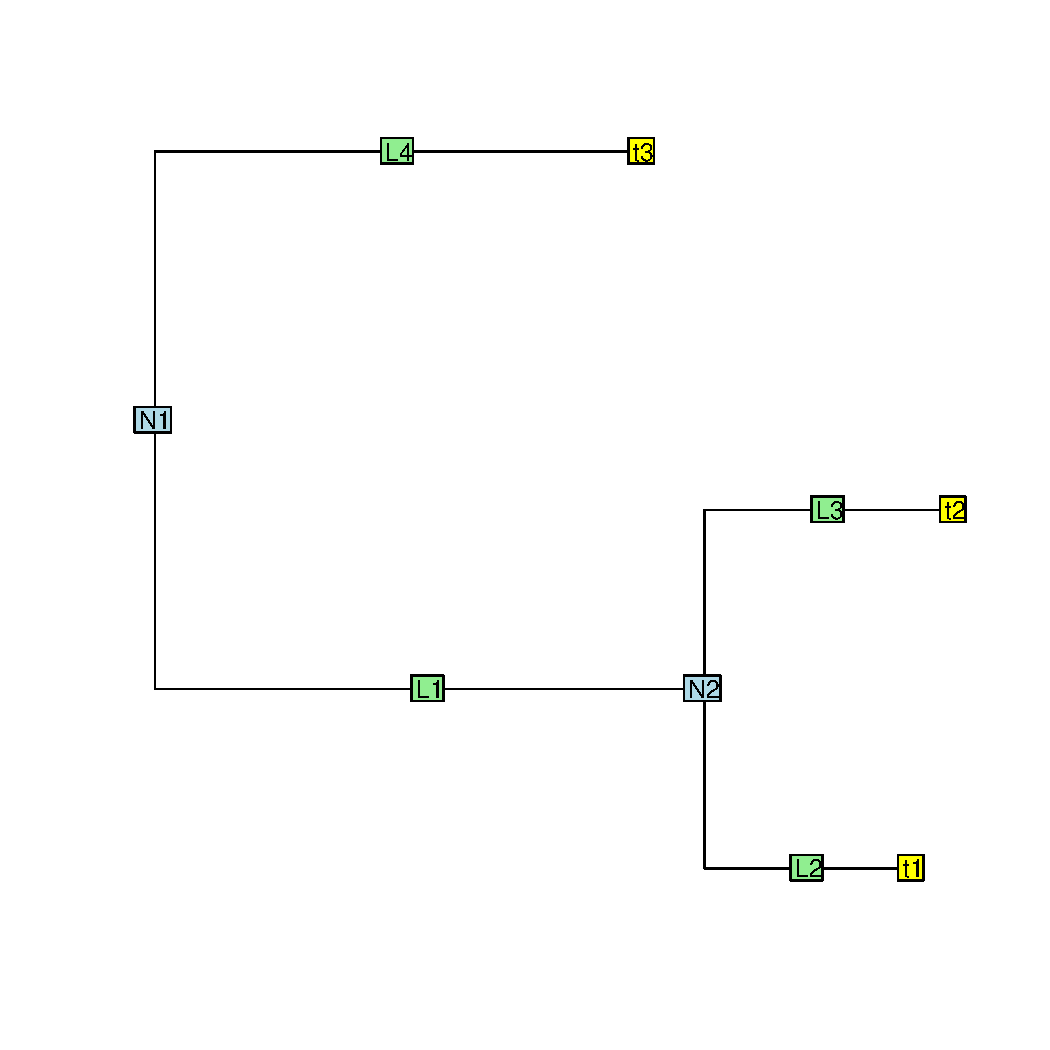
\includegraphics[scale=0.8,page=1]{./git_push/tree.pdf}
  \caption{\bmb{caption ??}}
\label{fig:tree}
\end{figure}
\end{center}

\begin{align*}
\bS = \begin{bmatrix}
\ell_1 \e_1 & \ell_2 \e_2 & 0 & 0 \\
\ell_1 \e_1 &  0 & \ell_3 \e_3 & 0 \\
0  &  0 & 0  & \ell_4 \e_4
\end{bmatrix}
\end{align*}
The error value corresponding to tip 1 is $\ell_1 \e_1 + \ell_2 \e_2$, where $\ell_i$ is the square root of the branch length $L_i$ in figure \ref{fig:tree} and the $\ell_i$ are independent, homoscedastic Normal variates with zero mean and $\sigma^2$ variance (i.e. variance for tip 1 is $(\ell_1 \e_1 + \ell_2 \e_2)^2 = (\ell_1^2 + \ell_2^2)\sigma^2$, linear in branch length) 

\subsubsection*{Constructing the species--branch random effects model matrix}

The $\bS$ matrix is the matrix product of an $n \times b$ indicator matrix $\bS_{ind}$ of branch indices, and a branch length vector $\bell$.

\begin{align}
\bS_{ind} = \begin{bmatrix}
1 & 1 & 0 & 0 \\ 
1 & 0 & 1 & 0 \\ 
0 & 0 & 0 & 1
\end{bmatrix} , 
\bell = \begin{bmatrix}
\ell_1 \\
\ell_2 \\
\ell_3 \\
\ell_4 
\end{bmatrix}
\label{eq:S}
\end{align}.
$\bS_{ind}$ is a binary (indicator) matrix that describes whether a particular branch occurs in the history of a focal species. 
$\bS \bS^T$ gives the variance-covariance matrix of the phylogeny. 

The random-effect model matrix $\bZ$ can be decomposed into term-wise model matrix $\bZ_{i}$ as described in \citet{bates2015fitting}.
Thus, the phylogenetic correlated random-effect matrix $\bZ^{C}_{i}$ is

\begin{equation}
\bZ^{C}_{i} = (\bS^{T}_{i}\bJ^{T}_{i} \ast \bX^{T}_{i})^{T}, \label{eq:ZC}
\end{equation}
where $\ast$ is the Khatri-Rao product \citep{khatri1968solutions}, $\bS_{i}$ is the $m_{i} \times b_{i}$ species--branch matrix; $\bJ_{i}$ is the $n_i \times m_i$ indicator matrix of grouping factors; $X_{i}$ is the $n \times p_{i}$ raw random effects model matrix. 


\mli{move example to the supp}
For example, using the phylogeny above (figure \ref{fig:tree}), if we begin with a raw model matrix,

\begin{align}
\bX = \begin{bmatrix}
1 & t_1  \\ 
1 & t_2  \\ 
1 & t_3 
\end{bmatrix} 
\end{align}
then the term-wise phylogenetic random effects model matrix is,

\begin{align}
\bZ^{C}_{i} = (\bS^{T}_{adji}\bJ^{T}_{i} \ast \bX^{T}_{i})^{T} =
\Bigg[
\Bigg(
\begin{bmatrix}
\ell_{adj1} & \ell_{adj1}  & 0 \\
\ell_{adj2} &  0  & 0 \\
0  &  \ell_{adj3} & 0 \\
0 & 0 &  \ell_{adj4} 
\end{bmatrix}
\begin{bmatrix}
1 & 0  & 0 \\
0 & 1  & 0 \\
0 & 0  & 1  
\end{bmatrix}
\Bigg)
\ast
\begin{bmatrix}
1   & 1   & 1  \\ 
t_1 & t_2 & t_3
\end{bmatrix} 
\Bigg]^T
\\
= \begin{bmatrix}
\ell_{adj1} & \ell_{adj1}t_1 & \ell_{adj2} & \ell_{adj2}t_1 & 0 & 0 & 0 & 0 \\
\ell_{adj1} & \ell_{adj1}t_2 & 0 & 0 & \ell_{adj3} & \ell_{adj3}t_2 & 0 & 0 \\
0 & 0 & 0 & 0 & 0 & 0 & \ell_{adj4} & \ell_{adj4}t_3
\end{bmatrix}
\end{align}


% 
% The scaled species--branch matrix $\bS_{adji}$ is scaled version of $\bS$ via the standardized generalized variance (SGV).
% SGVs are used as an intrinsic/natural way to scale down the variance-covariance matrix measured in different scales (for example, phylogenetic distance, years and etc) compariable to other variation in the model \citep{sengupta1987tests}.
% SGV is the $nth$ root of the generalized variance (GV), or the determinant of the variance-covariance matrix, where GV measures the overall size or volume of the variance-covariance matrix.  
% The SGV is given by:
% \begin{align}
% \bomega & = \textrm{det}(\bSigma_{phy})^{1/n},
% \end{align}
% where $n$ is the number of species in the phylogeny.
% 
% The analog in the $\bS$ is to scale the branch vector $\bell$ by square root of the SGV:
% \begin{align}
% \bell_{adj} & = \frac{\bell}{\sqrt{\bomega}}
% \end{align} 
% and the $\bS_{adj}$ is the matrix product of $\bS_{ind}$ and $\bell_{adj}$.

\subsection{Simulation}

We generated test data based on the simple mixed model formulation (\ref{eq:glmm1}, \ref{eq:glmm2}, \ref{eq:glmm3}, \ref{eq:glmm4} ) with a single response variable $\bY$ and a single predictor continuous variable $\bX$ for $n$ = 25, 50, and 100 species.
For wider range of comparisons, we simulate one observation ($X_i,Y_i$) per species.
For single-site model, the full simulation model is the following:
\begin{align}
\bY & = (\beta_0 + b_{phy_{int}}) + (\beta_1 + b_{phy_{slope}}) X + e_{residual}  \label{eq:ss_sim}\\\
(b_{phy_{int}}, b_{phy_{slope}}) & \sim \textrm{MVN} \Bigg( 0, \begin{bmatrix}
\sigma^2_{phy_{int}} & \sigma_{phy_{int},phy_{slope}} \\ 
\sigma_{phy_{int},phy_{slope}} & \sigma^2_{phy_{slope}}
\end{bmatrix} 
\Bigg) \\ 
e_{residual} & \sim \textrm{MVN} ( 0 , \Sigma) .
\end{align}
The model contains two fixed effect parameters ($\beta_0$ and $\beta_1$), three random effect parameters (phylogenetic random intercept variance, phylogenetic random slope variance and covariance between phylogenetic random slope and intercept) and observation/residual variance.  
Predictor and intercept level random effect of species are not applicable in this simulation setting with single observation per species because it will be confounded with the observational level variation (residuals).

We extend the simulation model by adding multiple sites where each site has one observation per species. The multiple-site full model is the following: 
\begin{align}
\bY & = (\beta_0 + b_{phy_{int}} + b_{sp_{int}} + b_{site}) + (\beta_1 + b_{phy_{slope}} + b_{sp_{slope}}) X + b_{sp:site} + e_{residual} \label{eq:ms_sim}\\
(b_{phy_{int}}, b_{phy_{slope}}) & \sim \textrm{MVN} \Bigg( 0, \begin{bmatrix}
\sigma^2_{phy_{int}} & \sigma_{phy_{int},phy_{slope}} \\ 
\sigma_{phy_{int},phy_{slope}} & \sigma^2_{phy_{slope}}
\end{bmatrix}
\Bigg) \\
(b_{sp_{int}}, b_{sp_{slope}}) & \sim \textrm{MVN} \Bigg( 0, \begin{bmatrix}
\sigma^2_{sp_{int}} & \sigma_{sp_{int},sp_{slope}} \\ 
\sigma_{sp_{int},sp_{slope}} & \sigma^2_{sp_{slope}}
\end{bmatrix}
\Bigg) \\
b_{site} & \sim \textrm{MVN} ( 0 , \Sigma_{site}) \\
b_{sp:site} & \sim \textrm{MVN} (0, \textrm{Kron}(\bf{I}_{site}, \sigma^2_{phy})) \\
e_{residual} & \sim \textrm{MVN} ( 0 , \Sigma)
\end{align}
The multiple-site full simulation model has five additional random effects (predictor and intercept level random effect of species variance and their covariance, random intercept of site and random intercept of species-site interaction) compared to the single--site full model.
Predictor and intercept level random effect of species are now applicable in the multiple-site model because there are multiple (one in every site) observations per species. 
Random intercept of species--site interactions examines whether the species within a comunity are likely to contain stronger phylogenetic relatedness than expected by chance; which is equivalent to phylogenetic attraction described in \cite{helmus2007separating}. 

\subsection{Platforms}

Our algorithmic approach is general and could be implemented in a wide range of computational platforms that support independent latent variables as part of a linear or generalized linear model. 
We implemented our approach using the R packages \pkg{lme4} \citep{bates2015fitting} and \pkg{glmmTMB} \citep{brooks2017glmmTMB}.
We compare our approach with five other R packages that can fit phylogenetic comparative models: \pkg{nlme} \citep{pinheiro2014r}, \pkg{phylolm} \citep{ho2014phylolm}, \pkg{pez} \citep{pearse2015pez}, and \pkg{brms} \citep{burkner2016brms}.
% \bmb{I think nlme can do other evolutionary models as well? May not be worth mentioning ...}
% \begin{verbatim}
% grep("\\.",apropos("^cor[A-Z]",ignore.case=FALSE),
% invert=TRUE,value=TRUE)
% \end{verbatim}
Phylogenetic generalized least squares (PGLS) (\code{gls} in \pkg{nlme}) is one of the most widely used techniques in phylogenetic comparative analysis; it is simily fitting a linear model where the covariance structure between species is the expected Brownian motion evolution process (or other evolutionary process) on the tree instead of independent and identically distributed. 
Phylogenetic generalized linear models (PGLM) (\code{phyloglm} in \pkg{phylolm}) is a slightly more flexible variation of PGLS that can allow additional observational residuals and also non-Gaussian response variables.
Both packages can model other evolutionary processes and different correlation structures (i.e. Pagel's $\lambda$, Blomberg's $K$ etc.), but we restrict our PGLS fits to the simple BM correlation. 
Neither PGLS nor PGLM can handle multiple observations or predictor level variation.
One of the relatively few packages that currently fit phylogenetic correlations to predictor level variation is \pkg{pez} (and very recently \pkg{phyr}), which can handle adding additional uncorrelated random slopes and interactions with intercept.
Lastly, bayesian phylogenetic GLMM using Markov chain monte carlo (MCMC) are avalible and can handle all cases described above. 
However, MCMC is often computationally expensive for GLMMs compared to platforms using optimization.
\pkg{MCMCglmm} \citep{hadfield2010general} is the most commonly used bayesian phylogenetic GLMM, but we will use \pkg{brms} instead, which uses a more powerful MCMC technique called Hamiltonian Monte Carlo (HMC) \citep{duane1987hybrid} that is more efficient \citep{li2018fitting}.
 
% Table \mli{ref something} provides the statistically equivalent fitting capabilities of common/existing phylogenetic methods.

% \begin{table}
% \begin{center}
\begin{table}
\begin{tabularx}{\textwidth}{|c||c|c|c|c|c|c|}
\hline
Package	& \small{nlme}	& \small{phylolm}	& \small{lme4/glmmTMB} & \small{pez} & \small{brms} & \small{MCMCglmm} \\
\hline
\hline
Single Site & X & X & X & & X & X \\
\hline
Phylo intercept & X & X & X &  & X & X \\
Phylo slope &  &  & X &  & X & X \\
Phylo correlation &  &  & X &  & X & X \\
Residual & & X & X &  & X & X \\
\hline
\hline
Multiple Site &  &  & X & X & X & X \\
\hline
Phylo intercept &  &  & X & X & X & X \\
Phylo slope &  &  & X & X & X & X \\
Phylo correlation &  &  & X &  & X & X \\
Phylo interaction & &  & X & X & X &  \\
Species intercept & &  & X & X & X & X \\
Species slope & & & X & X & X & X \\
Species correlation & &  & X &  & X & X \\
Residual & &  & X & X & X & X \\
\hline
\end{tabularx}
% \vspace{1in}
% ditto with site interaction								& ditto above $\mid$ sp:site		& ditto above \\
% \end{center}
\caption{bla bla bla \label{model_variant}}
\end{table}

\subsection{Simulation and evaluations}
We simulated 100 phylogenetic trees for each sample size (25,50,100, 500) and incorporated with simulation parameters (illustrated in figure 2 and 5) to simulate responses via the simulation model (\ref{eq:ss_sim}, \ref{eq:ms_sim}).
All model variants via different platforms were used to fit each realization.
Tables \ref{model_variant} shows the parameters that are estimable for each platform. 
All model must pass its respective convergence test before evaluating goodness of fit. 
For bayesian GLMM, we combined two convergence criteria to assess convergence: we required a value of the
Gelman and Rubin statistic and an effective sample size (ESS) greater than 1000 for each replication. 
For each replication we sample two chains starting with 10000 iterations. 

We used coverage to assess model fit.
Coverage refers to the frequency with which the computed confidence intervals include the true values of
parameters.
We used 90\% (Wald and profile) confidence intervals and quantile-based intervals (for bayesian GLMM)
to evaluate coverage.
We also compare computational speed between different platforms.

\section{Results}

\begin{center}
\begin{figure}[h]
  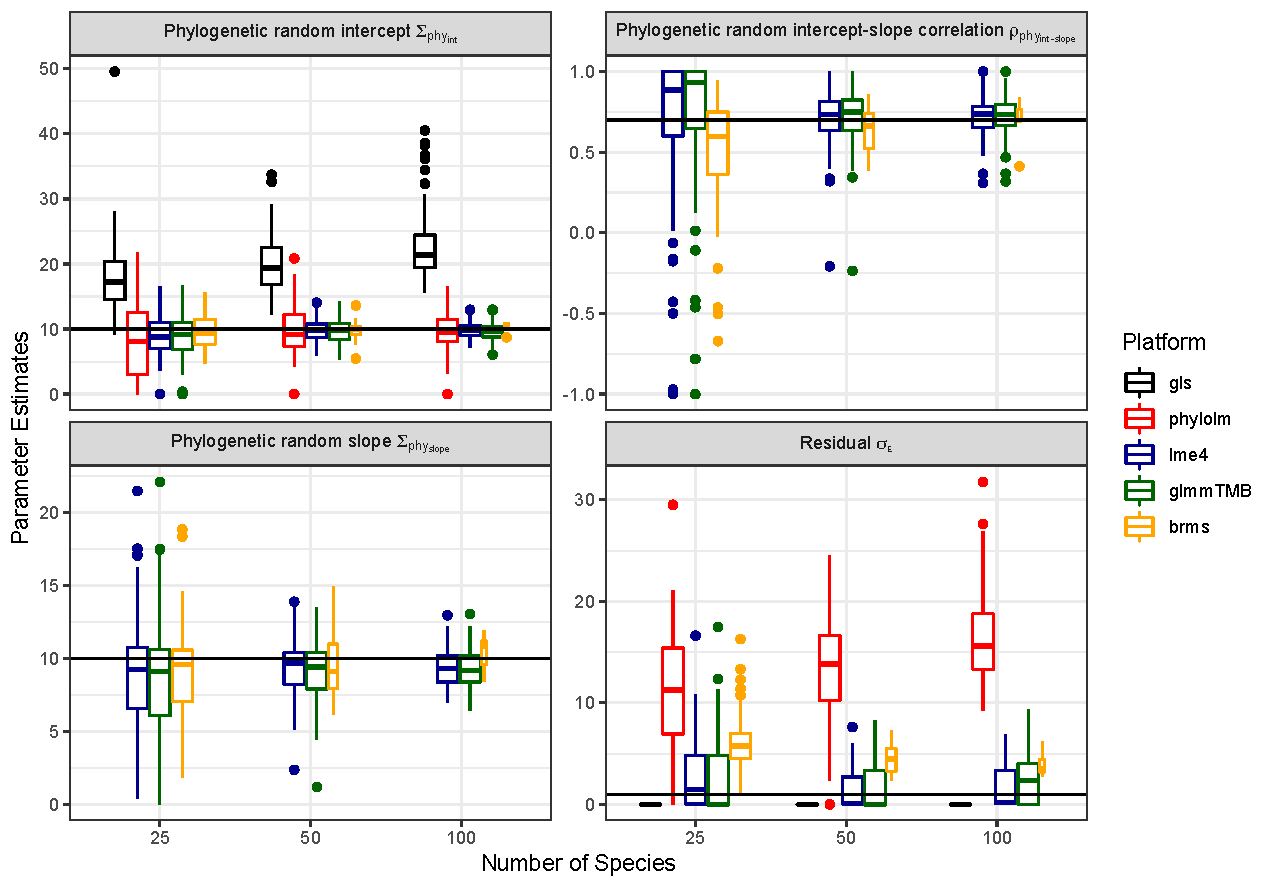
\includegraphics[scale=0.8,page=1]{./figure/ssplot.pdf}
  \caption{New}
\label{ssplot}
\end{figure}
\end{center}


\begin{center}
\begin{figure}[h]
  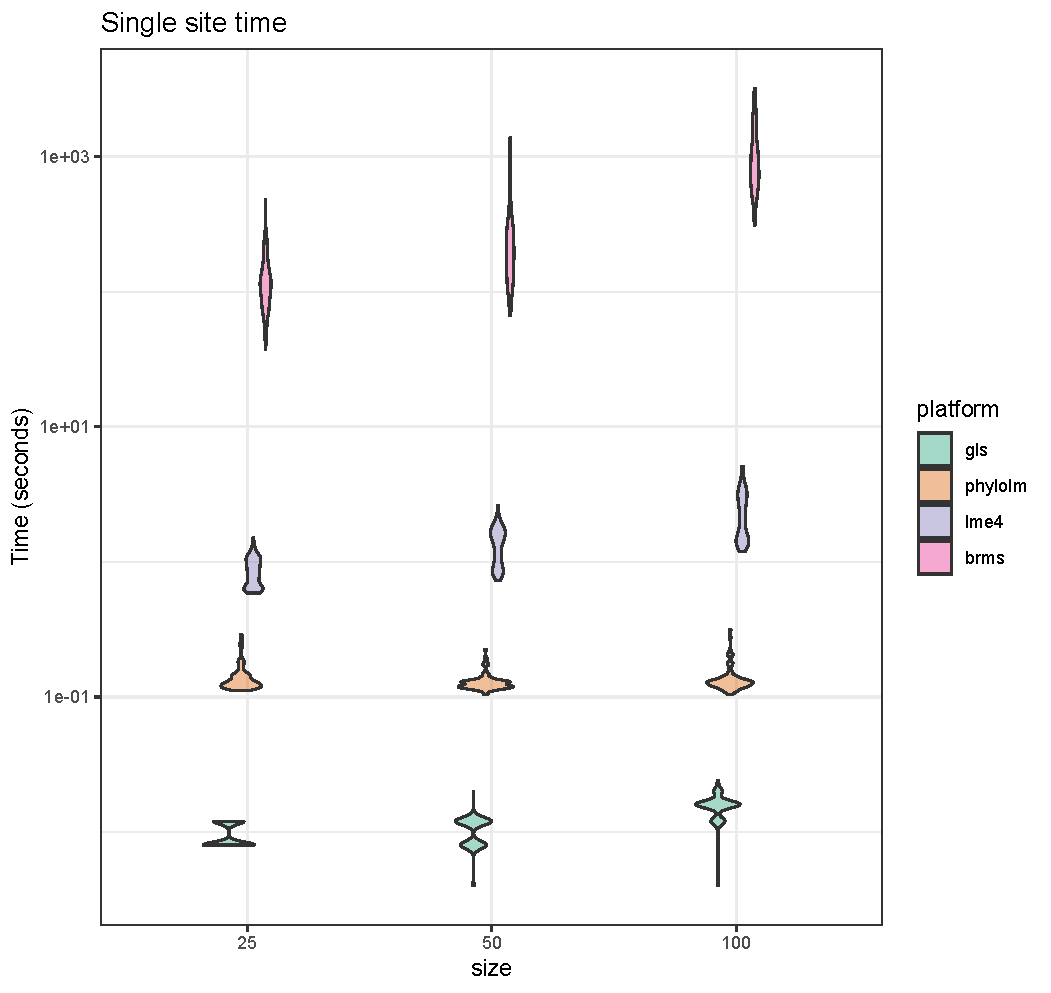
\includegraphics[scale=0.8,page=1]{./figure/sstime.pdf}
  \caption{New}
\label{ssplot}
\end{figure}
\end{center}


\begin{center}
\begin{figure}[h]
  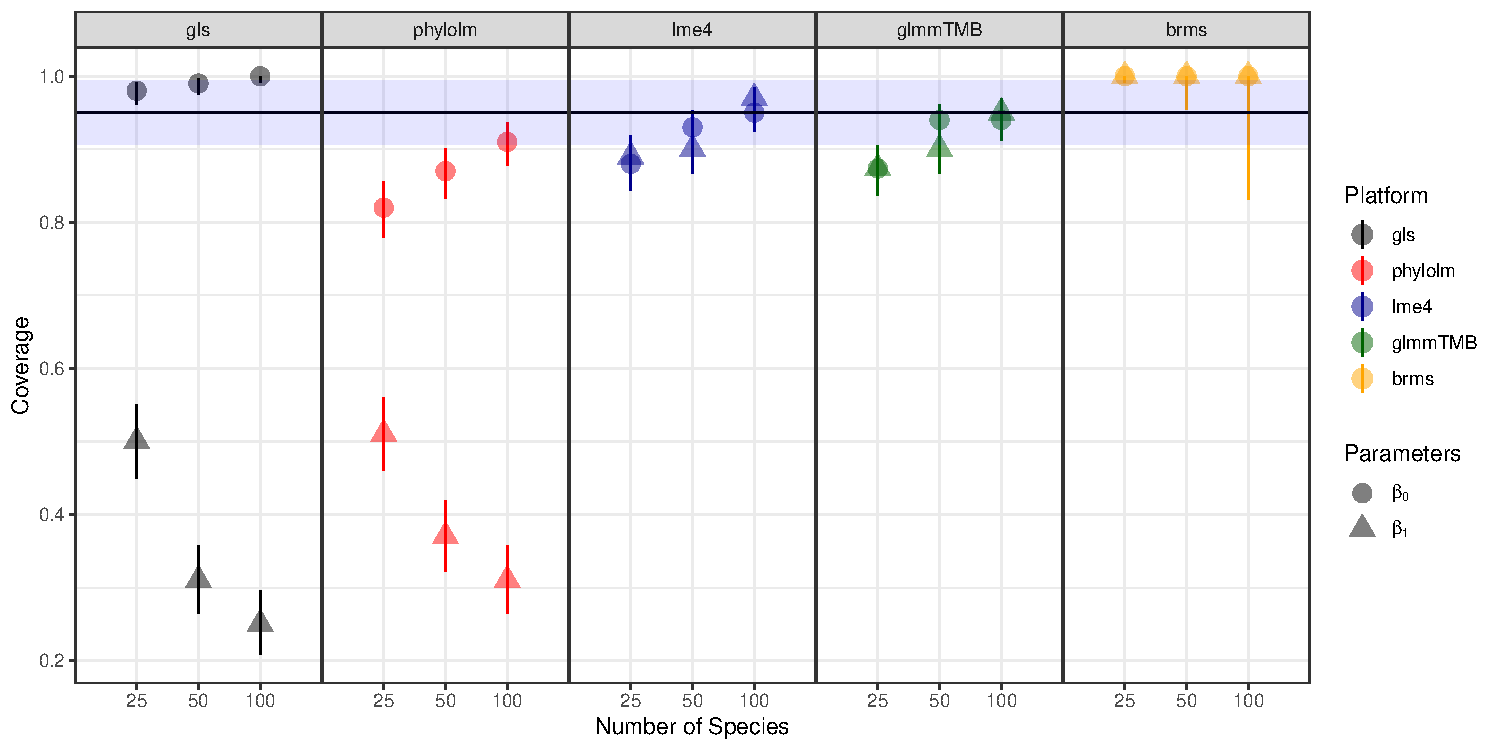
\includegraphics[scale=0.8,page=1]{./figure/sscoverage.pdf}
  \caption{New}
\label{ssplot}
\end{figure}
\end{center}


% \bmb{Need to think a little harder about the important points/order here (might be time to do the exercise where you take the results and boil them back down to short bullet points, in order to figure out whether you've said the important stuff, in the right order). Maybe lead by saying that all platforms give similar answers - to the extent that they are fitting the same statistical model (this might even be emphasized/explained above, in Methods). Am I correct in believing that phylolm=\pkg{lme4} but without intercept/slope correlation, and gls is additionally missing random slopes?}

\bmb{add refs to figures \ldots}

% \begin{itemize}
% \item{full model provides good estimates (except for correlation)}
% \item{reduced models try to fit with whatever parameters they have available (over-estimates the simulation parameters)}
% \item{no slope vs slope}
% \item{no correlation vs correlation}
% \item{as size/data/number of species increase, the parameter estimates gets better}
% \item{single site models are fast}
% \item{estimates gets closer to simulation parameter as number of species increase}
% \item{lme4/tmb are fast, everything else is slow for multiple sites}
% \end{itemize}

The full single site model using phyloglmm (which matches the single simulation model that incorporates phylogenetic intercept, slope and correlation) provides good estimates for all parameters except the random correlation parameter ($\sigma_{phy_{int},phy_{slope}}$). 
Fixed effect parameters ($\beta_0$ and $\beta_1$) estimates approaches nominal coverage as number of species increases for \pkg{lme4} and \pkg{glmmTMB} but not others.

In general, models that cannot match the simulation model (PGLM and PGLS) will try to fit the data with the parameters available. 
PGLM (which lacks the phylogenetic slope parameter) provides reasonable good estimates for phylogenetic intercept parameter ($\sigma_{phy_{int}}$) but overestimates the residual/observation standard deviation of the intercept ($\beta_0$) estimates slightly undercover the nominal coverage (95\% with 100 species) and have a bad coverage ($<$ 60\%) for the fixed slope parameter.
PGLS, with only one parameter available, confounds all variations (phylogenetic intercept, slope and residual variation) into the single parameter (phylogenetic intercept), resulting in overestimating the phylogenetic intercept and overcovering for $\beta_0$, and undercovering for $\beta_1$.

% \bmb{(2) please define ``robustness'' -- usually means lack of sensitivity to model.  Are you talking about the variance of the estimates? I'd prefer not to use ``robust'' in a non-standard way if possible (2) what are small/medium/large? I see that $n=\{20,100,500\}$ and $m=\{1,20\}$, but not sure how these match up to ``small'', ``medium'', ``large''; is Figure 1 all $m=1$? Might be worth just labeling by $n=??$ rather than using small/medium/large}
% It is unclear how different levels of phylogenetic signal are being confounded under the error free (without tip variation) assumption for the PGLS models.
% \bmb{can we figure this out, even in an empirical/crude way??? it's tough to have results without knowing the true value they're aiming for ...}


\begin{center}
\begin{figure}[h]
  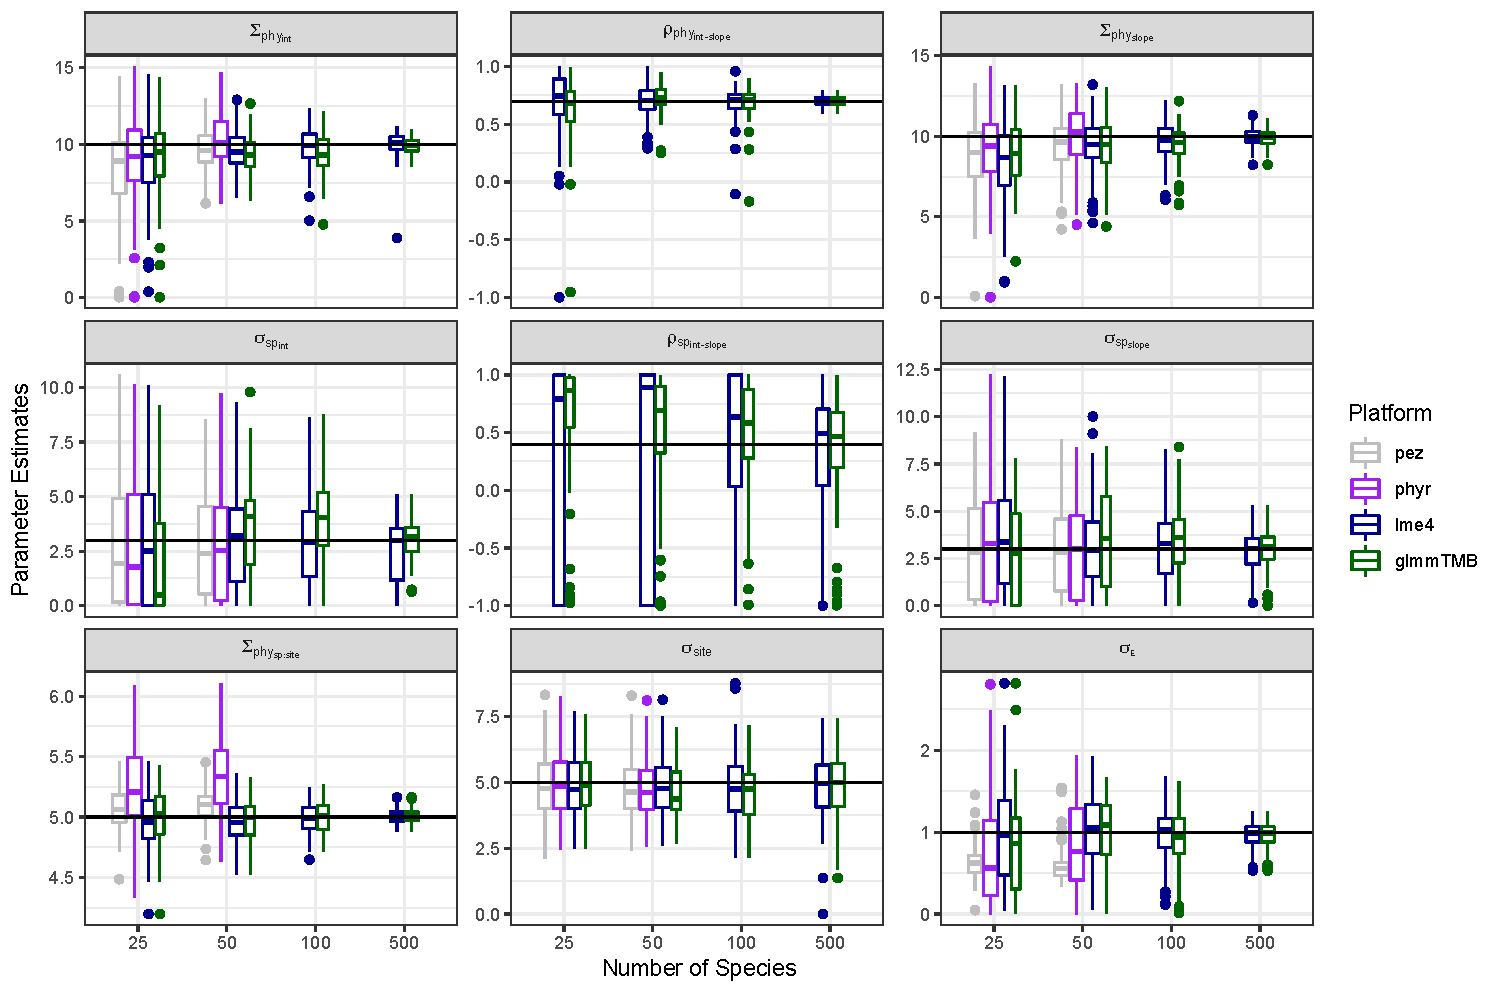
\includegraphics[scale=0.8,page=1]{./figure/msplot.pdf}
  \caption{new}
\end{figure}
\end{center}


\begin{center}
\begin{figure}[h]
  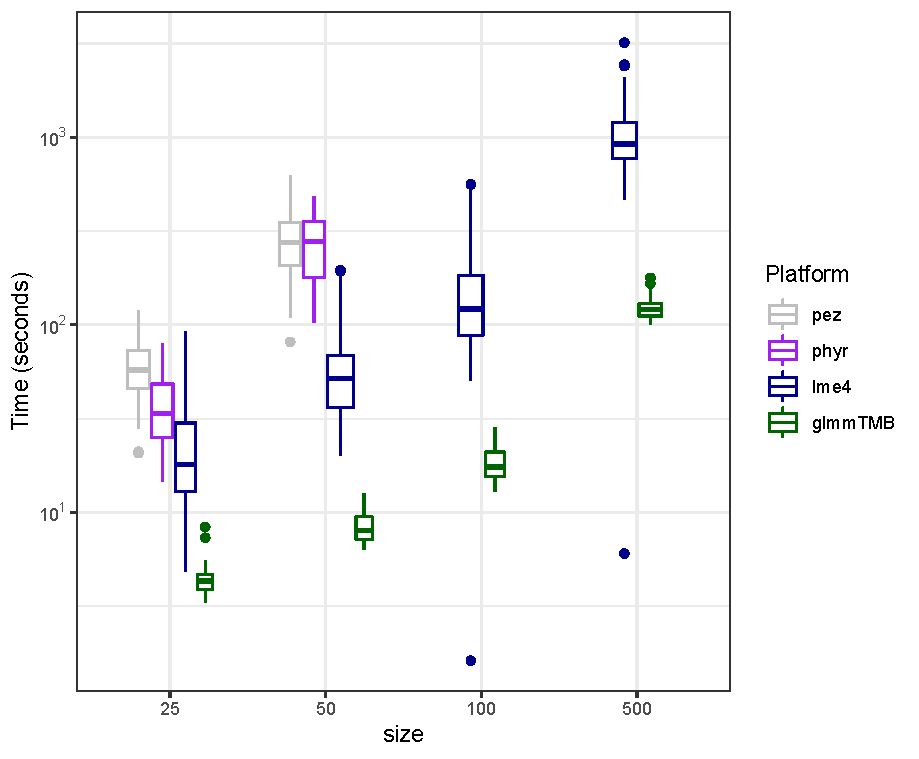
\includegraphics[scale=0.8,page=1]{./figure/mstime.pdf}
  \caption{new}
\end{figure}
\end{center}


\begin{center}
\begin{figure}[h]
  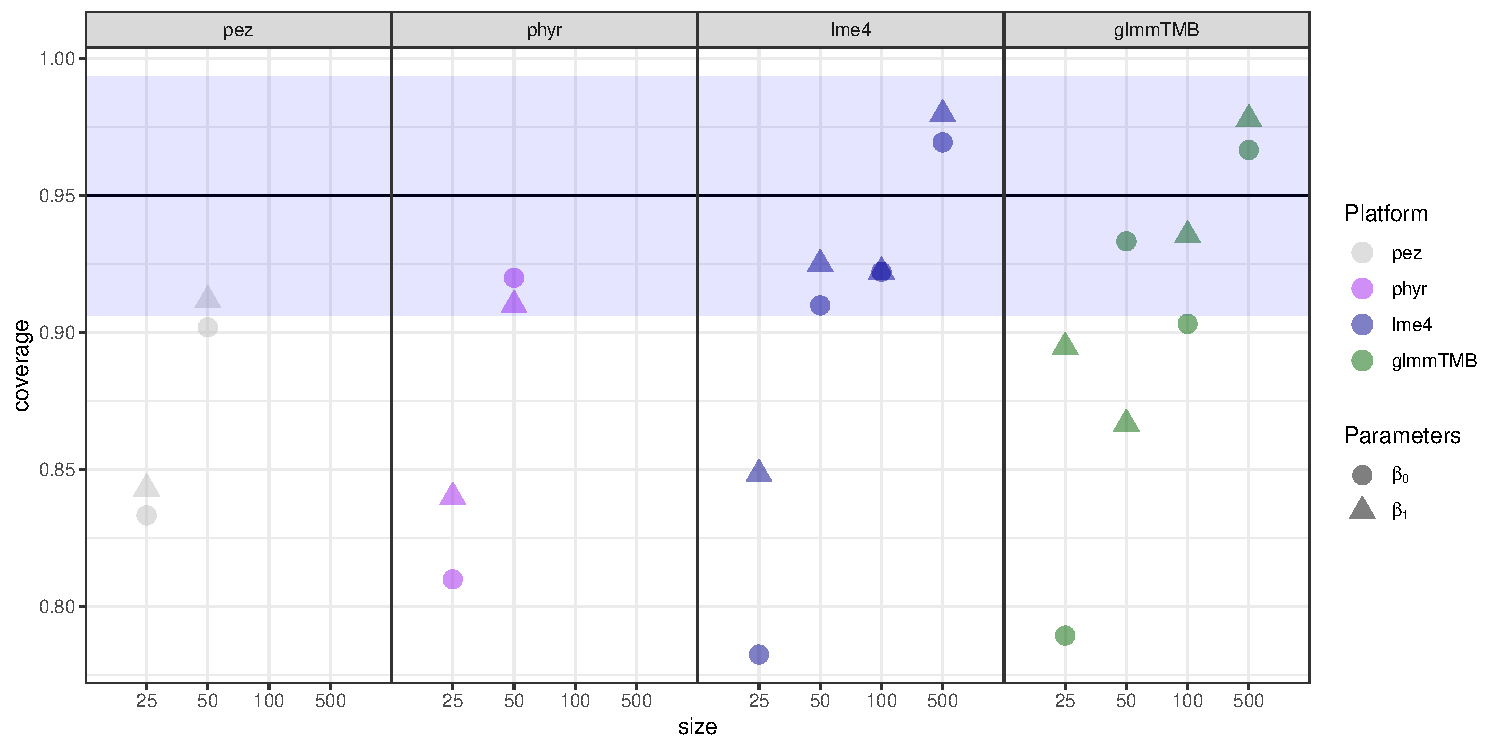
\includegraphics[scale=0.8,page=1]{./figure/mscoverage.pdf}
  \caption{new}
\end{figure}
\end{center}


Multiple site fits on the other hand, are much more similar across platforms (as the fitted and simulation models are more similar).
Similar to the single site fits, \pkg{lme4} and \pkg{glmmTMB} which matches the simulation model provides good estimates for all parameters except for the random correlation parameter ($\sigma_{sp_{int,slope}}$).
The lack of correlations in \pkg{pez} and \pkg{phyr} statistical models does not appear to have a large effect on its ability to estimate other parameters, whereas \pkg{pez} underestimates (lower estimates) many parameters.  
% \bmb{Can you identify the extreme cases in \pkg{lme4}'s estimate? Are these singular models? Would they be diagnosable? Can you say anything about when the assumption of independence of slope and intercept \textbf{would} be a problem? (If you can think of such a scenario, you could run sims for one such example - don't need to go into great detail, but being able to say that you confirmed that it's a problem in such-and-such a case would be important.)}
% \mli{save it for random slope discussion}

However, despite the similarities of parameter estimates across platforms for the multiple sites simulation fits, the efficiency (measured by computational speed) are different across platforms and sample size.
For example, the median time for \pkg{lme4} to fit 50/100 species model takes $~$ 50/100 seconds versus $~$ 200/2000 seconds for \pkg{pez} and \pkg{phyr}. 
Lastly, it takes $\sim$ 1000 seconds for lme4 to fit 500 species model; it was not practical for \pkg{pez} and \pkg{phyr} to fit 500 species for our study, where the computational speed did not scale linearly with sample size 25/50/100.
\pkg{glmmTMB} is almost an order of magnitude faster than \pkg{lme4}.

% \bmb{Can you put a lower bound on \pkg{pez}'s computation time? How long did you take to give up? How does it scale? can you either figure out from first principles
%   or (easier) do a brute-force series of increasing sample size and
%   compute a log-log regression of time vs sample size to find the
%   approximate power?}

We used our method and fitted the full model of the dune meadow data recently used with \pkg{pez} \cite{li2017canfun}. 
We have obtained identical results for fix and random effect estimates, our code is approximately 120 times faster than \pkg{pez}. 
Codes for fitting dune meadow analysis using \pkg{lme4} and \pkg{pez} are provided in the supplements. 

\newpage

\section{Discussion}


% \bmb{say something about the implications of this [e.g. good enough for getting an overall impression of phylog. whatever-it-is but not enough for detailed description/inference about the evolutionary process?] (or maybe that should be saved for the Discussion?)}

The evolutionary model simulations presented in this paper are an oversimplification of real evolutionary processes in nature, but it is analogous to how researchers fit models to study complicated systems (as it is impossible to create a model to "match" the complexities of nature).
We have fitted models using different platforms that best match the simulation models. 
Models that cannot match the simulation (full) model are expected to underperform; it is important to understand the limitations and performance of these simpler models that are restricted by the commonly used methods available.
Using models that include some form of phylogenetic variation and residual variation is necessary to detect evolutionary process.
Here are a few points researchers should think about when fitting phylogenetic regression models.

\subsection{Process and residual (observation) variabilities and confoundings}

\bmb{explain: classical scenario for PIC is when we have species-level data (i.e., species averages or ``typical'' values).  What do we do when we have multiple observations per species?  Why can't we just average? (cf. \cite{murtaugh2007simplicity}) with a nested, balanced design, averaging by group and doing 1-way ANOVA gets the same answer for fixed effects as LMMs). \textbf{answers}: (1) unbalanced data (can handle by weighting by $n$, equivalent to assuming homoscedasticity and using inverse-variance weights); (2) non-Gaussian responses (averaging doesn't make sense) [can we use offsets to handle this case? don't know]; (3) maybe for equivalent of randomized block designs? (4) when within-species variance is actually of interest}
Process and observation errors are highly confounded in phylogenetic regression if it is not handled correctly. 
For single measurement per species model, any method that can account for at least two sources of variation (one for the residual variance, and at least one for the process variation) will be sufficient to a first approximation (i.e. Pagel's $\lambda$, Blomberg's $K$).
If multiple observations are allowed per species, then using methods such as Pagel's $\lambda$ can potentially incorrectly estimate the amount of phylogenetic process by substituting tip variation with residual variation. 
However, one can summarise multiple measurements to a single measurement (for example, mean or median) per species to avoid confounding residual and tip variations.

\subsection{Random Slopes}

\bmb{I think you need a lot more here; what does a random slopes model mean? You have one sentence that says ``people should be thinking about random slopes''. Then you talk about correlation (which is a much more subtle/less important issue, I think).}
In classic GLMM (without phylogenetic relationships), random slopes models are not always appropriate, but they are relevant over a wider range of scenarios than people are currently thinking about \cite{schielzeth2008conclusions, cleasby2015quantifying,ord2010adaptation}.
Neglicting random slopes can lead to erroneous fixed effect estimates \citep{schielzeth2008conclusions} (parameters of interest) as shown in the simulations above. 
When analyzing relationships among species between traits and environmental variables, it is entirely plausible that change in effect of predictor variables have on traits are changing in a phylogenetically correlated way.
In fact, it is easier to interpret random slopes in the evolutionary process context (i.e, are size of different species phylogenetically correlated, or growth rate through time of different species phylogenetically correlated?)
It may be easier to simplify the phylogenetic relationships (at the random slopes level) and think about the random-slopes model in a strictly hierarchical setting (i.e., estimating different slopes for each family, or taxon \citep{bunnefeld2012island}) - the PGLMM collapses to a standard random-slopes model. 
Users should be aware of two important questions when fitting random-slope models: How much data do we need in order to practically estimate the random slopes? and Are we making a mistake by ignoring random slopes \citep{schielzeth2008conclusions}? 
% However, in the PGLMM context, as long as there's variation in the predictor among tips, there will be variation among taxa at some level, so random-slopes models will (almost always) be \emph{theoretically} identifiable.


\subsection{Extension and alternatives}

Our analysis covers the classical phylogenetic comparative methods (i.e. phylogenetic least squares, linear and mixed models).
Even within the scope there is additional room for exploration we neglected, such as exploring phylogenetic multivariate response models, non-BM evolution processes (such as Ornstein-Uhlenbeck (OU) process which accounts for both selection and drift processes \cite{butler2004phylogenetic}), Bayesian approaches \cite{hadfield2010general}.
More broadly, the simple independence error approach we developed here offers a more efficient and mathematical equivalent way to do Brownian motion evolution process phylogenetic comparative analysis. 
This approach can in principle be combined flexibly with the state of the art phylogenetic mixed models using platforms that supports independent latent variables such as \pkg{MCMCglmm} \citep{hadfield2010mcmc}; a widely used Bayesian approach to PGLMM.
However, in principle just like GLMM and most statistically models, users should be aware the amount of data they have and the complexity of the model they want to fit (i.e. What should we do when we don't have enough data? Should we use a complex model and overfit \citep{barr2013random}, the right balance of complexity and data \citep{baayen2008mixed} or possibility of Bayesian approaches \cite{hadfield2010mcmc}).
More importantly, this implementation in \pkg{lme4} allows users to fit phylogenetic mixed models to the fullest ( that other frequentist platforms lack of (i.e. large data, unbalanced species observations, complex random effects) and explore new ideas.


\section{Conclusion}

We have presented a simple approach to fit phylogenetic mixed models that is both more efficient and statistically equivalent approach and comparison of classical PCM to simulated data. 
First, this new approach is magnitudes faster compared to existing phylogenetic mixed models without losing robustness/accuracy and can easily combined with any statistically mixed model framework. 
Last and most importantly, it is more flexible in fitting large phylogenies, large volume of data, unbalanced data sets, and complex random effects such as slope correlations.

\newpage

\section{Supplements -- translation}

$1 \mid Sp_{phylo}$, $0 + X_{E} \mid Sp_{phylo}$ and $X_{E} \mid Sp_{phylo}$ means phylogenetically related have similar response,   

\begin{tabularx}{\textwidth}{|l|X|X|}
\hline
Formula & Statistics & Biology \\
\hline
$1 \mid Sp$ &
random species intercept; variation within species in mean response across all factors &
variation of how species respond \\
\hline

$0 + X_{E} \mid Sp$ &
random slope of environment factor within species; variation in coefficient within species for the environmental factor &
variation of how species respond to the same environmental factor \\
\hline

$1 + X_{E} \mid Sp$ &
random slope of environmental factor within species with correlated intercept; variation in coefficient within species for the environmental factor with correlated mean response across all other factors &
variation of how species respond in the same environmental factors and the correlation of the variation of how they respond in general \\
\hline

$1 \mid Site:Sp $ &
random variation in intercept among species within sites &
variation of how species respond within sites \\
\hline

$1 | Sp_{Phylo} $ &
variation among species in mean response across all factors demonstrate phylogenetic signal &
phylogenetically related species respond similarly \\
\hline

$0 + X_{E} \mid Sp_{Phylo}$ &
variation among species for environmental factors demonstrate phylogenetic signal &
phylogenetically related species respond similar (share common response) to the same environmental factor \\
\hline
\end{tabularx}
            
            
            
            
            
                                                              


\bibliography{phyloglmm}

\end{document}

